\documentclass[12pt, a4paper]{article}


%%%%%%%%%%%%%%%%%%%%%%%%%%%%%%%%%%%%%%%%%%%%%%%%%%%%%%%%%%%%%%%%%%%%%%%
%%-----------------------VYUŽITÉ PACKAGES----------------------------%%
%%%%%%%%%%%%%%%%%%%%%%%%%%%%%%%%%%%%%%%%%%%%%%%%%%%%%%%%%%%%%%%%%%%%%%%
\usepackage[czech]{babel}
\usepackage{geometry}
\usepackage[final]{graphicx}
\usepackage{anyfontsize}
\usepackage{setspace}
\usepackage{hyperref}
\usepackage{subcaption}
\usepackage{listings}
\usepackage{color}
\usepackage{float}
\usepackage[T1]{fontenc}
\usepackage{amsmath}

\hypersetup{
    colorlinks,
    citecolor=black,
    filecolor=black,
    linkcolor=black,
    urlcolor=black
}

% Code Snippets %
\definecolor{dkgreen}{rgb}{0,0.6,0}
\definecolor{gray}{rgb}{0.5,0.5,0.5}
\definecolor{mauve}{rgb}{0.58,0,0.82}

\lstset{frame=tb,
  language=Java,
  aboveskip=3mm,
  belowskip=3mm,
  showstringspaces=false,
  columns=flexible,
  basicstyle={\small\ttfamily},
  numbers=none,
  numberstyle=\tiny\color{gray},
  keywordstyle=\color{blue},
  commentstyle=\color{dkgreen},
  stringstyle=\color{mauve},
  breaklines=true,
  breakatwhitespace=true,
  tabsize=3
}

%%%%%%%%%%%%%%%%%%%%%%%%%%%%%%%%%%%%%%%%%%%%%%%%%%%%%%%%%%%%%%%%%%%%%%%%%%%%%
%%-----------------------ZAČÁTEK VLASTNÍHO TEXTU---------------------------%%
%%%%%%%%%%%%%%%%%%%%%%%%%%%%%%%%%%%%%%%%%%%%%%%%%%%%%%%%%%%%%%%%%%%%%%%%%%%%%
\begin{document}

\begin{titlepage}
	\title{
		\vspace{-4cm}\hspace{-10cm}
		
\includegraphics[width=8cm]{assets/logo.png} \\
		\vspace{5cm}
		\begingroup
		\setstretch{4}\fontsize{30}{10}\selectfont\fontdimen2\font=0.8ex
		\parbox{13.3cm}{
			\centering{\textbf{KIV/PPR - Semestrální práce}\\
				\fontsize{24}{10}\selectfont\centering{{Hledání vzorce korelace mezi datovými řadami}}
			}}
		\endgroup}
	\date{}
	\author{}
	\maketitle \thispagestyle{empty}
	\vspace{3cm}
	\hspace{0cm}\parbox[b][5cm][b]{8cm}{{\setstretch{1.5}
				Autor: Bc. Jan Hereš\\
				Datum: 27.12.2023\\
				Poslední úprava: \today\\}}
\end{titlepage}
\newpage


\tableofcontents
\newpage

\section{Zadání}
\paragraph{} ,,Cílem práce je najít vzorec pro korelaci mezi 3D akcelerometrem a srdečním tepem. 
Z \href{https://physionet.org/content/big-ideas-glycemic-wearable/1.1.2/}{\underline{tohoto odkazu}} si stáhněte příslušnou část datových souborů - HR a ACC soubory. 
Vstupní časové řady normujte pomocí vláken. 
Pak napište jednoduchý generátor funkcí s následujícím prototypem:

\begin{center}
  \begin{verbatim}
    double transform (const double acc_x, const double acc_y, 
    const double acc_z);
  \end{verbatim}
  \label{code-transform}
\end{center}

Pro výslednou časovou řadu spočítejte její korelaci se srdečním tepem. 
Čím menší hodnota, tím lepší korelace. 
Tím vlastně dostanete fitness funkci, pokud budete generovat těla transformační funkcí evolučním/genetickým algoritmem, jako to např. dělá genetické programovaní nebo gramatická evoluce. 
Tento algoritmus vektorizujte.
Celý výpočet spusťte na OpenCL zařízení - tj. nemusíte psát parser výrazů, ale OpenCL driver to udělá za vás. 
Je vhodné, aby se výpočet míry korelace a transformace odehrál celý na GPU, čímž se pak vyhnete zbytečnému kopírování dat.
Ve finále vyberte transformační funkci s co největší korelací a tu zobrazte v grafu společně se srdeční frekvencí. 
Graf vygenerujte jako .svg.''
(Zadání bylo převzato z oficiálních Courseware stránek předmětu)

\newpage
\section{Analýza zadání, související studie a naměřených dat}

\subsection{Analýza zadání}
Jako absolutně prvním úkolem při řešení tohoto problému byla důkladná analýza zadání a souvisejících faktů. 
Nejdříve se tedy budeme zabývat samotným zadáním z CW. 
Hlavní cíl práce: \textbf{Najít vzorec pro korelaci mezi 3D akcelerometer a srdečním tepem}.
K dispozici máme \textbf{dvě sady} dat - jedna z akcelerometru a druhá ze senzoru srdečího tepu.
Z toho tedy vyplývá, že je potřeba data prozkoumat - formát, velikost, variabilita, \dots (blíže v kapitole \ref{chapter-data-analysis})
Data je třeba \textbf{normalizovat} (tzn. mapování na hodnoty v intervalu <0, 1>).
Tento proces by měl být probíhat \textbf{vícevláknově}.
Dále je potřeba vytvořit funkci, která bude \textbf{transformovat} data z akcelerometru do dat srdečního tepu, ideálně se zadaným prototypem (viz \ref{code-transform}).
Pro tato data je pak potřeba spočítat \textbf{korelaci} s původními, naměřenými daty srdečního tepu.
Spočtenou korelaci pak můžeme porovnat s původní a dle toho \textbf{minimalizovat/maximalizovat} (v závislosti na interpretaci) \textrightarrow \textbf{fitness funkce} pro případ, pokud budeme k řešení využívat koncepty gramatické evoluce či genetického programování.
Tento algoritmus by měl být \textbf{vektorizován}.
\textbf{Celý výpočet} by měl probíhat na \textbf{OpenCL zařízení}.
Výsledky pak budeme exportovat do formátu \textbf{SVG}.

\paragraph{} V předchozím odstavci jsou \textbf{tučně} vyznačeny klíčové činnosti a aspekty, které by měl program respektovat.
Díky této rychlé a jednoduché analýze lze již teď sestavit hrubou posloupnost činností, které bude potřeba implementovat

\begin{enumerate}
  \item Načtení naměřených datových sad (ACC, HR) - CPU, sekvenční
  \item Předzpracování dat (normalizace, případná interpolace) - CPU, paralelizace
  \item Výpočet korelace mezi naměřenými daty (fitness funkce) - CPU, vektorizace
  \item Výpočet transformační funkce - OpenCL (GPGPU)
  \item Výpočet korelace nových a původních dat - OpenCL (GPGPU)
  \item Min/Max na základě výsledků - OpenCL (GPGPU)
  \item Export původních a vygenerovaných dat do SVG - CPU
\end{enumerate}

\paragraph{} Tato posloupnost činností bude ještě v následujících kapitolách upravována na základě získaných znalostí v průběhu tvorby programu.

\subsection{Analýza související studie a naměřených dat}
\subsubsection{Analýza studie}
\paragraph{} Data poskytnutá jako zdroj k této práci jsou součástí studie dostupné na zmíněném odkaze.
Po důkladném pročtení této studie byla zjištěna následující důležitá fakta (zahrnuta pouze ta, která jsou zásadní pro tuto práci):

\begin{itemize}
  \item Subjekty byly ženy mezi 35. - 65. rokem věku ve stádiu post-menopauzy a naměřenou hladinou hemoglobinu \textit{HbA1c} mezi 5.2\% a 6.4\% 
  \item Data byla měřena v horizontu 10 dní
  \item Subjekty byly vybírány bez ohledu na rasu, sociální stav, barvu pleti a etnicitu a které vyjádřily souhlas s účastí v této studii
  \item Potencionální subjekty, které v minulosti prošly chronickou obstrukční plicní nemocí (COPD), kardiovaskulárním onemocněním, libovolnou rakovinou nebo chronickým onemocněním ledvin nejsou součástí této studie 
  \item Časová razítka v rámci poskytnutých dat byla upravena, aby nemohlo dojít k identifikaci subjektů
  \item Počet subjektů, pro něž byla poskytnuta naměřená data, je 16
  \item Data byla měřena chytrým náramkem \textit{Empatica E4} s následujícími vlastnostmi:
    \begin{itemize}
      \item Data z akcelerometru byla měřena s frekvencí 32 Hz
      \item Data ze senzoru srdečního tepu byla měřena s frekvencí 1Hz 
    \end{itemize}
  \item Naměřená data jsou poskytnuta s následující strukturou (csv):
    \begin{itemize}
      \item ACC: <timestamp, x, y, z>
      \item HR: <timestamp, hr>
    \end{itemize}
\end{itemize}

\paragraph{} Na základě zmíněných faktů lze tedy odvodit následující. Subjekty mají hladinu hemoglobinu A1c v \textbf{normální či míně zvýšené} \cite{Hemoglobin}, tudíž se dá očekávat přítomnost \textit{prediabetes} u některých subjektů.
Tento fakt bude důležitý zejména při vyvozování závěrů ze získaných výsledků (v případě, že bude tato práce dále pokračovat nad rámec předmětu KIV/PPR).
Co se týče konkrétně naměřených dat, můžeme díky způsobu výběru subjektů očekávat \textbf{standardní} hodnoty a průběh srdečního tepu (neočekáváme anomálie v naměřených datech).
Data obsahují časová razítka, z čeho vyplývá, že je možné zajistit časovou synchronizaci mezi sběry dat.
Očekáváme 16 ACC souborů a 16 HR souborů.
Data z akcelerometru byla měřena s odlišnou frekvencí, než data ze senzoru srdečního tepu, tudíž bude potřeba, v rámci procesu normalizace, sledovanou \textbf{periodu sjednotit}. 
Zde se naskýtá otázka jakou zvolit periodu? 
Jako první možnost se nabízí \textbf{perioda 1s}.
Toto bude výchozí nastavení programu, nicméně na základě získaných výsledků je možné sledovat i delší periody (například 10s či 30s).
Sledování delších period nám totiž umožní lépe sledovat projevy trend změn v akcelerometru, které se mohou, z logiky věci, projevovat v rámci zatížení srdečního organismu v rámci jednotek až desítek sekund. 
Naopak, sledováním dlouhé periody ztrácíme část informace o prudkých změnách. 

\newpage
\subsubsection{Analýza naměřených dat}
\label{chapter-data-analysis}
\paragraph{} Samotná naměřená data jsou k dispozici ve formátu \textit{csv}.
Jak již bylo řečeno, data naměřená z akcelerometru jsou v následujícím formátu: <timestamp, x, y, z>.
Je tedy zřejmé, že v rámci fáze načtení a zpracování dat bude nutné data správně ,,parsovat'' (stejná zásada bude platit i pro data ze senzoru srdečního tepu).
Důležitým aspektem jsou \textbf{mezní naměřené hodnoty}. 
Hodnoty z akcelerometru se pohybují v intervalu <-128.0; 127.0>, hodnoty ze senzoru srdečního tepu v rozsahu (0.0; 255.0).
Díky zjištění těchto rozsahů můžeme jednoduše zavést normalizační konstanty pro daná data (viz dále).
Největší soubor velikostně zabírá méně jak 1.1GB, což nám dává prostor pro optimalizace v rámci návrhu řešení (viz dále).

\begin{enumerate}
  \item Načtení naměřených datových sad (ACC, HR) - CPU, sekvenční
    \begin{itemize}
      \item Ověření přítomnosti zdrojových souborů
      \item Vytvoření datových struktur pro načtení obsahu souborů
      \item ,,Parsování'' a uložení dat
    \end{itemize}
  \item Předzpracování dat (normalizace, případná interpolace) - CPU, paralelizace
    \begin{itemize}
      \item Případná časová synchronizace vzorků
    \end{itemize}
  \item Výpočet korelace mezi naměřenými daty (fitness funkce) - CPU, vektorizace
  \item Výpočet transformační funkce - OpenCL (GPGPU)
  \item Výpočet korelace nových a původních dat - OpenCL (GPGPU)
  \item Min/Max na základě výsledků - OpenCL (GPGPU)
  \item Export původních a vygenerovaných dat do SVG - CPU
\end{enumerate}

\newpage
\section{Návrh řešení}
\subsection{Prvotní návrh řešení}
\paragraph{} V rámci požadavků v rámci předmětu KIV/PPR byla dne 10.10.2023 uskutečněna prezentace, obsahově se týkající prvotního návrhu řešení a analýzy.
Tato prezentace je dostupná ve složce \textit{doc/presentation} v rámci dodaného zdrojového archivu.
Společně s prezentací je v rámci tohoto archivu i dostupný prvotní diagram návrhu řešení. 
Tento diagram je vyobrazen na obrázku \ref{fig-control-flow-diagram}. 


\begin{figure}
    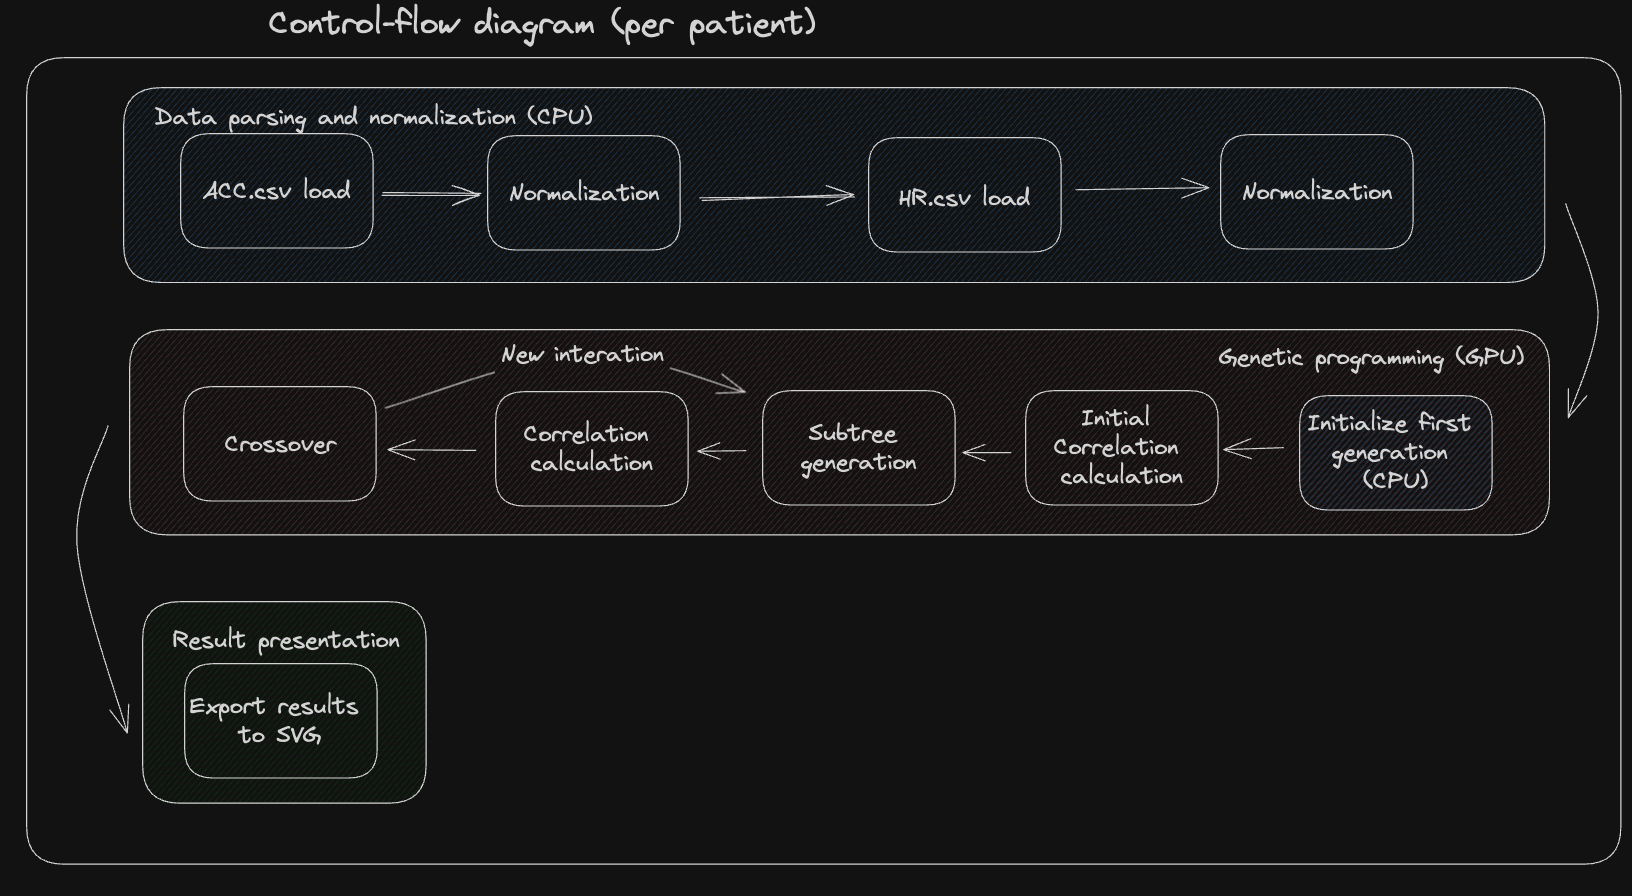
\includegraphics[width=\linewidth]{assets/ppr_diagram_p1.png}
  \caption{Diagram znázorňující návrh řešení}
  \label{fig-control-flow-diagram}
\end{figure}

\subsubsection{Popis diagramu}
\paragraph{} Celý diagram se dá rozdělit do tří zásadních fází: 
\begin{enumerate}
  \item Načtení a předzpracování dat 
  \item Zpracování a výpočet vzorce korelace
  \item Export vypočtených dat
\end{enumerate}

\paragraph{} V následujících odstavcích budou jednotlivé části diagramu podrobněji popsány.


\paragraph{Načtení dat} První nutnou činností je samozřejmě potřeba načíst zdrojová data. 
Jelikož se jedná o \textit{csv} soubory, budou čteny řádek po řádku v jednom vlákně. 
Přístup k souborům bude \textbf{sekvenční}, zejména z důvodu, že paralelní přístup ke čtení dat z disků rychlostně neškáluje v porovnání s tradičním sekvenčním přístupem (\textit{náhodné čtení}) v rámci tradičních souborových systémů (tj. NTFS, ext či APFS), respektive není autorovi v rámci jeho omezených znalostí známa studie, známa studie, která by tento fakt vyvracela.
Taktéž je ale prokázáno, že čtení dat ze starších disků s pohyblivými částmi (tj. HDD) paralelním způsobem snižuje celkový čtecí ,,výkon'', pokud se soubory nachází na fyzicky odlišných místech tohoto média, tudíž čtecí hlava stráví nezanedbatelnou část čtení čistě pro posun do správného bloku.
Samozřejmě tento vliv silně závisí na nesčetném množství dalších aspektů moderních souborových systémů a diskových medií, nicméně taková diskuze není předmětem této práce. 
Pro potřeby této práce pouze uvažujme tradiční sekvenční přístup ke čtení souborů, tedy v jednom okamžiku bude čteno pouze z jednoho souboru.
Pro každý soubor tedy platí stejné následující kroky. 

Soubory jsou čteny řádek po řádku, po přečtení řádky je automaticky proveden tzv. \textit{parsing}, tedy rozdělení dat dle příslušné struktury souboru.
Nejdříve je nutné zjistit, zda-li si \textbf{časová razítka} odpovídají.
Po porovnání razítek může dojít v zásadě ke dvěma situacím: razítka odpovídají, nebo jsou měřené vzorky časově posunuty.
V prvním zmíněném případě není třeba dalšího zásahu, nicméně pokud jsou jejich časová razítka rozdílná, je potřeba daný rozdíl v počtu záznamů přeskočit.

Po synchronizaci časových razítek jsou u souborů s hodnotami z akcelerometru v jednotlivých osách pohybu přidány do samostatných vektorů.
Zde je vhodné zmínit, že v rámci konzultace se zadavatelem práce byl umožněn alternativní přístup - posuzování korelace jednotlivých os \textbf{samostatně} vůči srdečnímu tepu.
Tento přístup umožní sledovat, zda-li se korelace v jednotlivých směrech pohybu liší, či nikoliv. 
Pro jednotlivé osy budou tedy vytvořeny samostatné vektory, do kterých budou ,,parsovaná'' data postupně vkládána.

U souborů s hodnotami ze senzoru srdečního tepu vzniká pouze jeden vektor, jelikož z logiky věci máme pouze jednorozměrná data. 
Zbývající postup je pak totožný s postupem pro soubory s daty z akcelerometru soubory.

\begin{figure}
  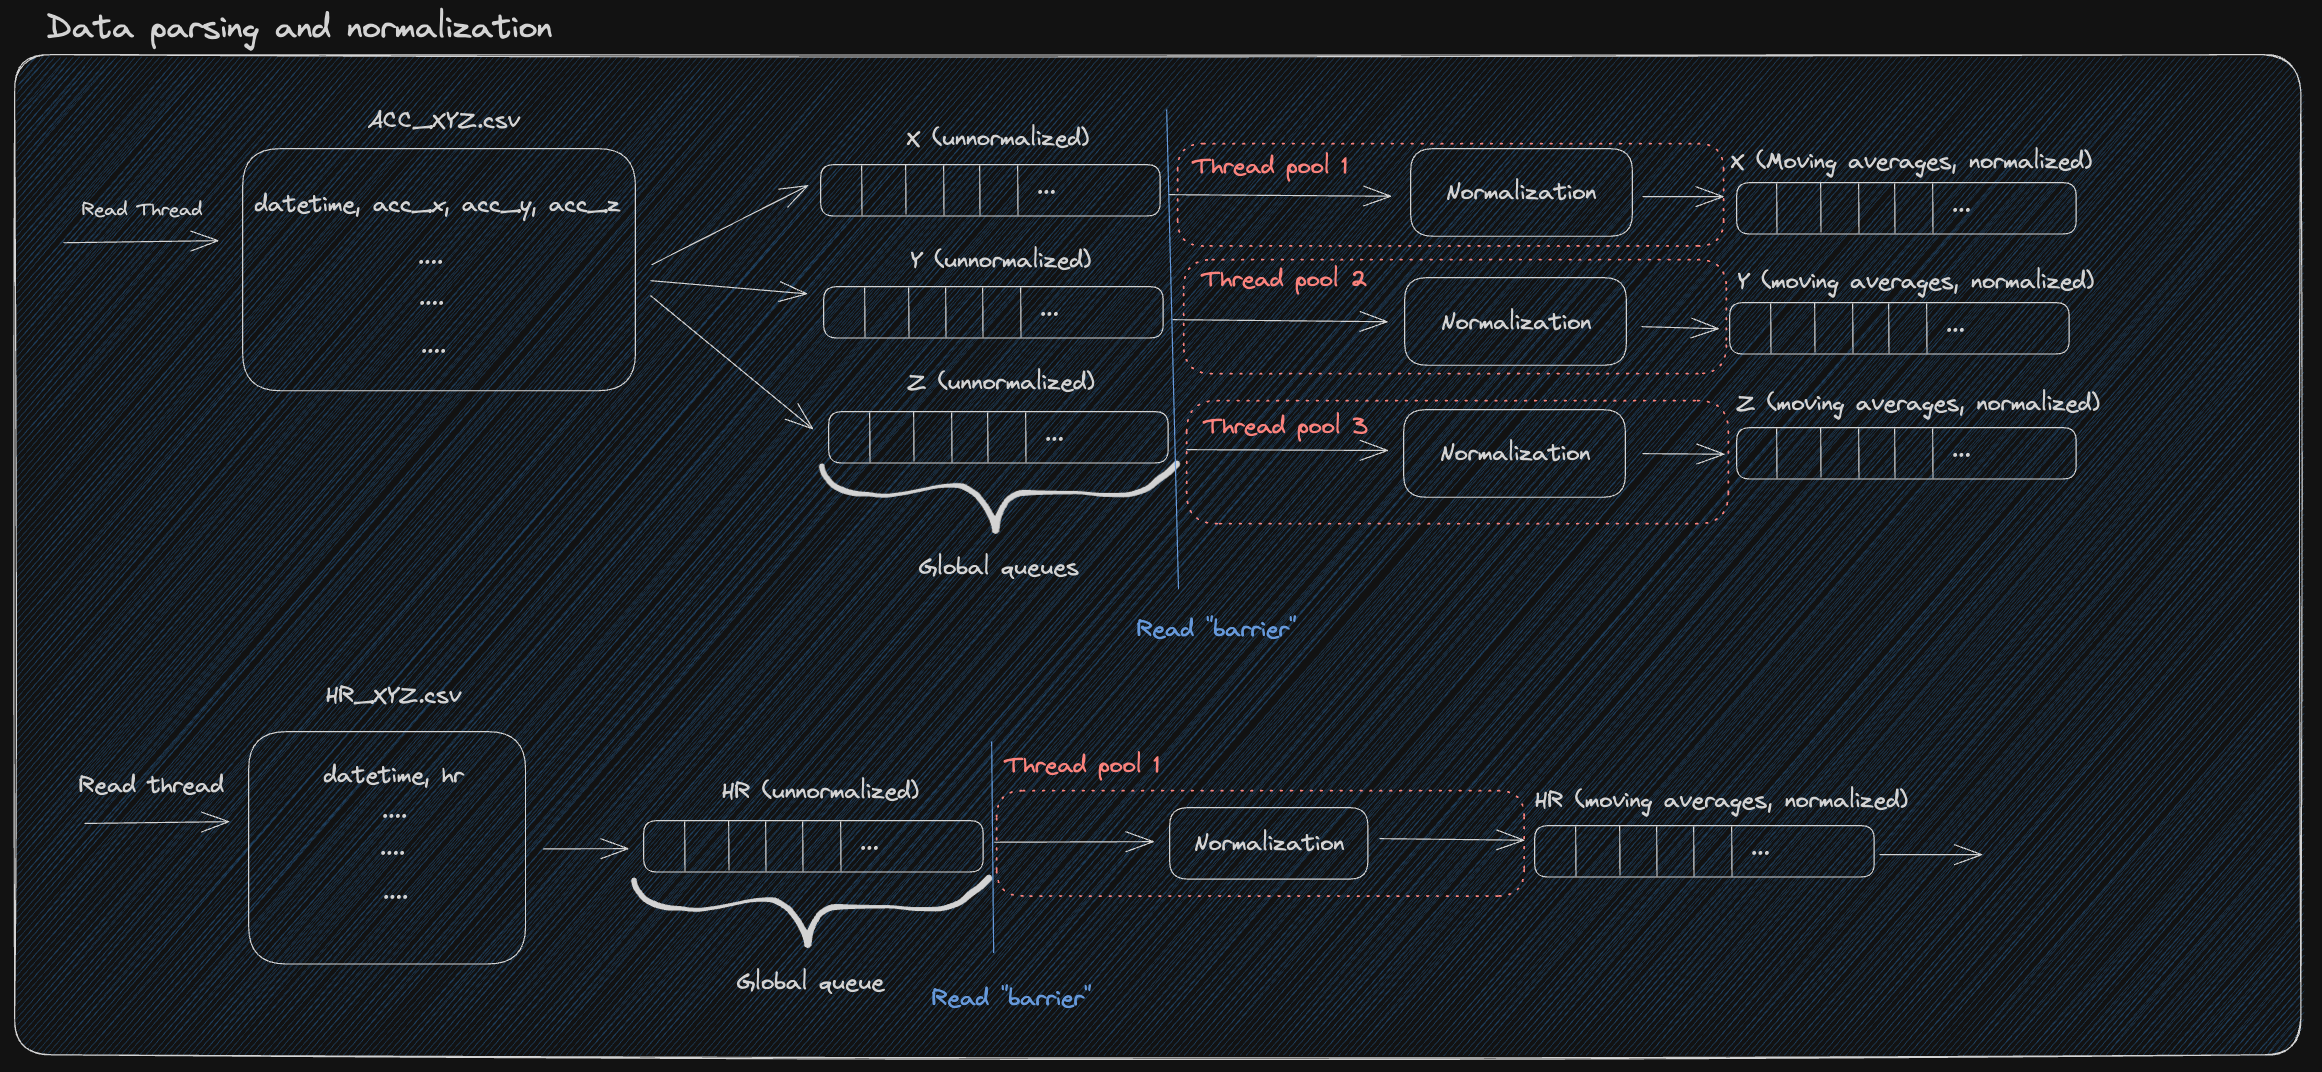
\includegraphics[width=\linewidth]{assets/ppr_diagram_p2.png}
  \caption{Diagram fáze načtení a předzpracování dat}
\end{figure}

\newpage
\paragraph{Předzpracování dat} Po načtení dat následuje fáze jejich předzpracování. 
V této fázi dochází zejména k jejich normalizaci. 
V rámci tohoto procesu jsou tedy data nejdříve sjednocena na společnou zvolenou periodu. 
Poté je v rámci této periody vypočten \textbf{klouzavý} průměr, jež je normalizován na interval <0;1>.

Poznámka: Normalizace vektorů reprezentující data z akcelerometru probíhá \textbf{paralelně} (tzn. všechny 3 vektory jsou normalizovány najednou). 

\paragraph{Výpočet prvotní korelace} 
Pro výpočet korelace využijeme \textbf{Pearsonova korelačního koeficientu}.
Základní vzorec pro tento výpočet je formulován níže: 

\begin{center}
  \begin{equation}
    \begin{aligned}
      r_{x, y} = \frac{E{[(X - u_x)(Y - u_y)]}}{\sqrt{E(X - u_x)} * \sqrt{E(Y - u_y)}} \\
    \end{aligned}
  \end{equation}

  alternativně 

  \label{eq-pearson-two-pass}
  \begin{equation}
    \begin{aligned}
      r_{x, y} = \frac{\sum_{i=1}^{n}{(x_i - \overline{x})(y_i - \overline{y})}}{\sqrt{\sum_{i=1}^{n}{(x_i - \overline{x})^2}} \sqrt{\sum_{i=1}^{n}{(y_i - \overline{y})^2}}}
    \end{aligned}
  \end{equation}
\end{center}


\paragraph{} Problém tohoto přístupu spočívá, že je pro jeho výpočet nutné znát průměrné hodnoty veličin X a Y, což implikuje nutnost dvojího průchodu daty.
Při hledání rychlejších alternativ byla nalezena studie, ve které je odvozen následující vztah: 

\begin{equation}
  \begin{aligned}
    \overline{x}^{'} = \overline{x} + \frac{x_{n+1} - \overline{x}}{n - 1} \\
    M_{2, X} = \sum_{i=1}^{n}{(x_i - \overline{x})} \\
    M_{2, X}^{'} = M_{2, X} + (x_{n + 1} - \overline{x})(x_{n + 1} - \overline{x}^{'}) \\
    C_{2, S}^{'} = C_{2, S} + \frac{n}{n+1}(x_{n+1} - \overline{x})(y_{n+1} - \overline{y}) \\
    r_{x, y} = \frac{C_{2, S}}{\sqrt{M_{2, X}} \sqrt{M_{2, Y}}} 
  \end{aligned}
\end{equation}

\paragraph{} Společnou výhodou je, že veličinu statistiky pro Y veličinu (v našem případě HR) je nutné spočítat pouze jednou, což zásadně redukuje výpočetní náročnost. 
Výhod tohoto upraveného algoritmu je hned několik.
Pro upravený vztah je nutnost pouze jednoho průchodu daty (tzv. \textbf{online} výpočet). 
To je vhodné zejména v případě, kdy by nebylo možné veškerá data načíst najednou (což ale není náš konkrétní případ). 

Nicméně se zde vyskytuje i jeden problém, kterým je netriviálnost efektivní paralelizace výpočtu.
Z toho důvodu bylo od původního návrhu pro využití upravené vzorce upuštěno a implementace bude využívat \textbf{základní vzorec} pro výpočet Pearsonova korelačního koeficientu.


\paragraph{Výpočet - algoritmus genetického programování} Navržený algoritmus získání vzorce korelace zakládá na konceptech \textbf{genetického programování}.
Mějme výchozí generaci skládající se z dvojic množin, jejichž každý prvek reprezentuje \textbf{úplný binární strom skládající se z jednoho kořene a dvou potomků}, vyobrazených na obrázku \ref{fig-starting-generation}.
Pro tento algoritmus definujeme následující množinu možných operací: 
\begin{itemize}
  \item Sčítání
  \item Odčítání
  \item Násobení
  \item Dělení
\end{itemize}
 
\paragraph{} Následně definujme možnou množinu operandů: 

\begin{itemize}
    \item $X_i$ reprezentující převzatou hodnotu z původních dat
    \item Libovolné reálné číslo z intervalu <0, 1>
\end{itemize}

\begin{figure}
  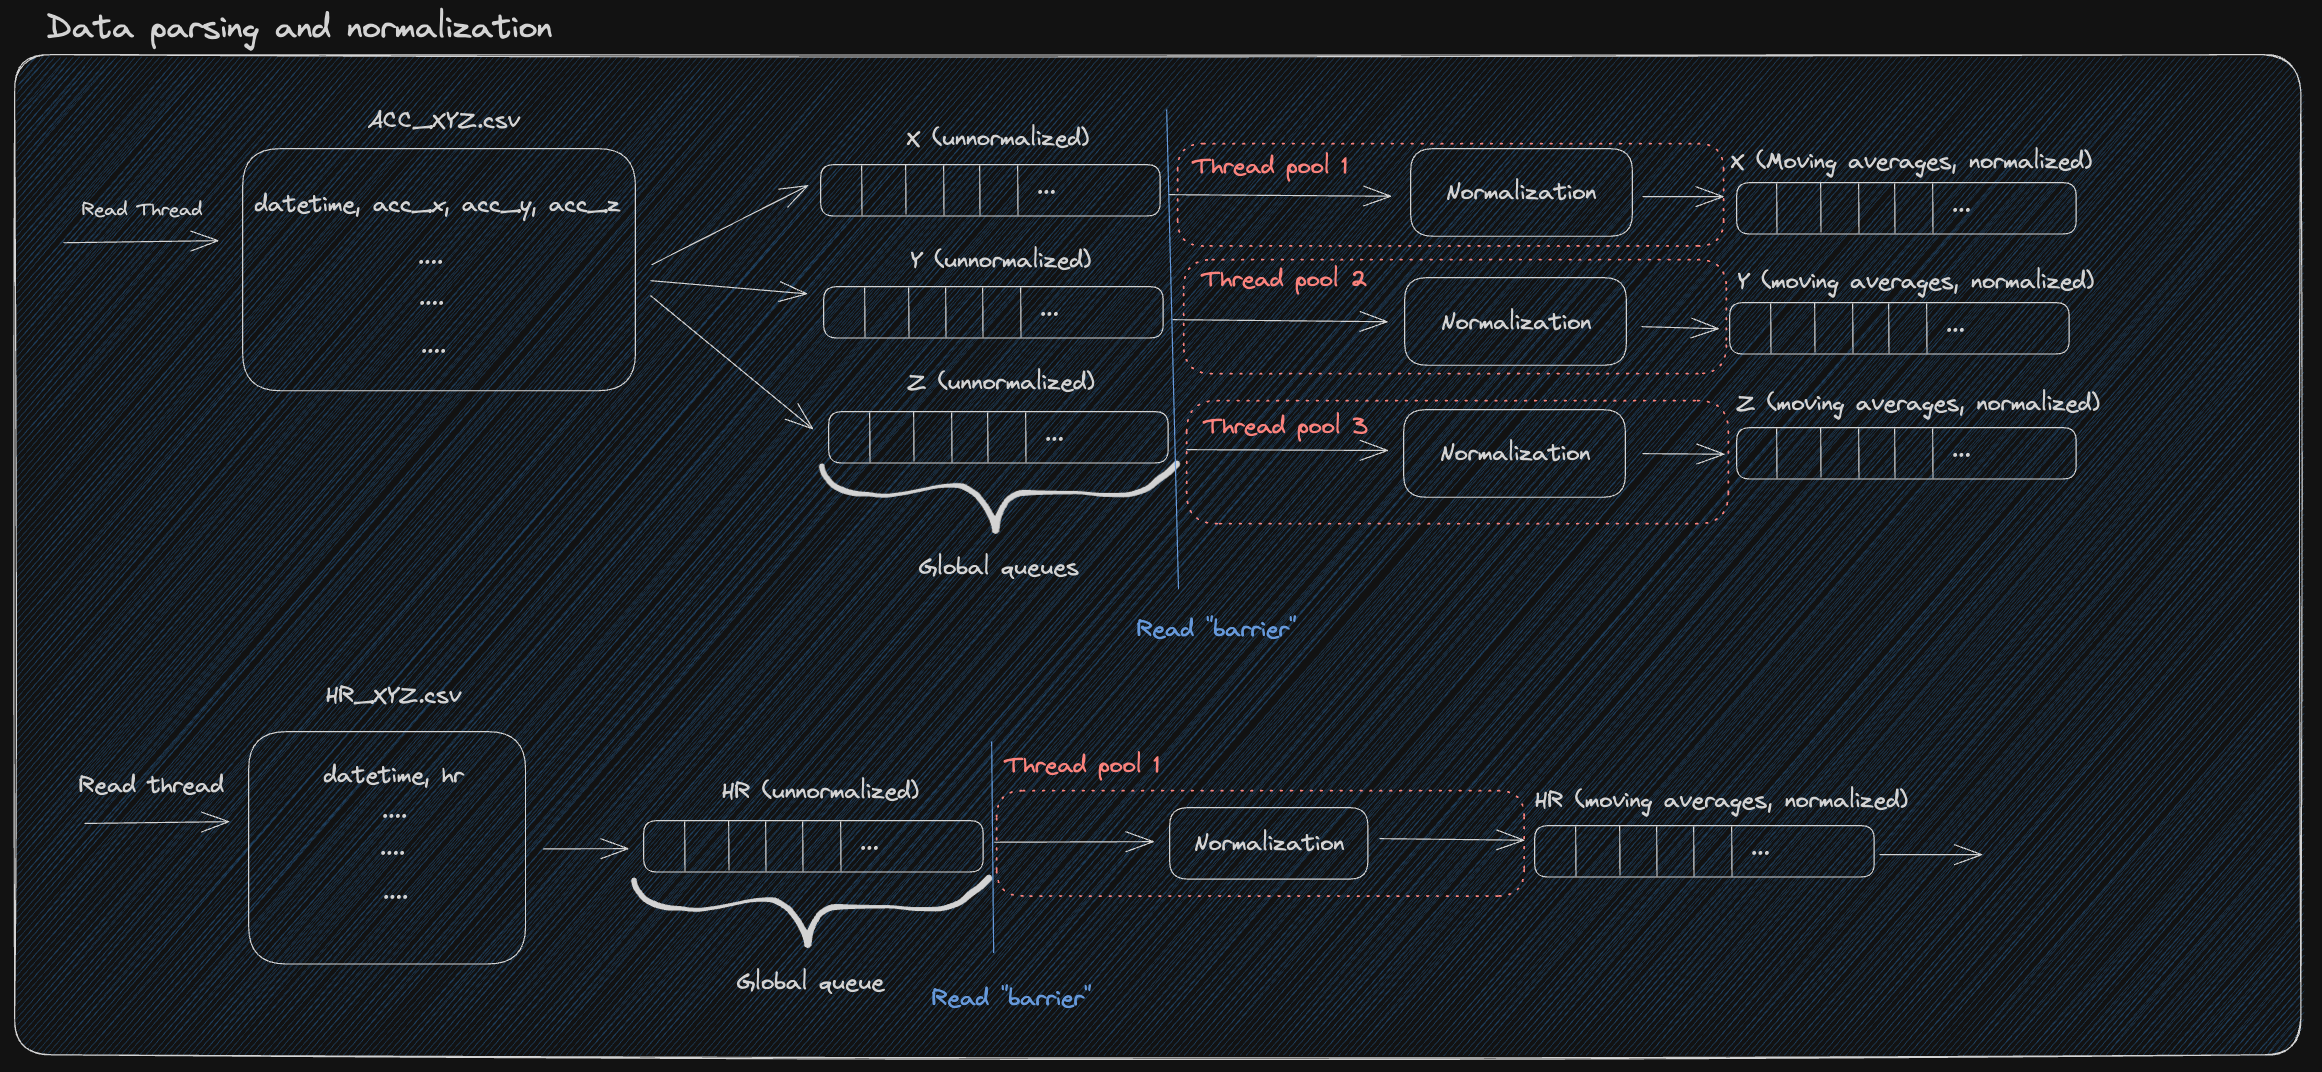
\includegraphics[width=\linewidth]{assets/ppr_diagram_p2.png}
  \caption{Výchozí dvojice jedinců navrženého algoritmu}
  \label{fig-starting-generation}
\end{figure}

\paragraph{} Algoritmus lze pak popsat následujícím postupem:

\begin{enumerate}
  \item Vytvořte prvotní generaci (viz obrázek \ref{fig-starting-generation})
  \item Náhodně vygenerujte množinu dalších uzlů až do maximální zvolené velikosti jedince
  \item Pomocí tohoto stromu reprezentující matematický výraz vygenerujte nové hodnoty srdečního tepu
  \item Spočítejte korelaci mezi vygenerovanými a původními daty 
  \item Pokračujte krokem dva po zvolený počet iterací
\end{enumerate}

\paragraph{} Poznámka: V algoritmu došlo k menší změně oproti návrhu uvedenému ve zmíněné prezentaci. 
Místo úlohy min/max samotné hodnoty korelace spočívá implementace v minimalizaci odchylky vůči původní korelaci.
Toto řešení bylo vybráno po delším uvažování nad konkrétní implementací původně navrženého algoritmu za účelem získání co nejpřesnějšího vzorce zachycující korelaci původních dat.

\paragraph{Export výsledků} Po získání vzorce korelace je vhodné výsledky zobrazit. 
Pro tento účel bude využito formátu SVG \cite{SVG}.

\section{Popis implementace}
\paragraph{} Implementační poznámky na začátek: Veškerá chybová hlášení a upozornění jsou dostupná v souborech \textit{warnings.hpp} a \textit{errors.hpp}.
Veškeré využité globální konstanty jsou deklarovány v souboru \textit{constants.hpp} a definovány v souboru \textit{constants.cpp}.
Při práci s datovým typem ,,string'' bylo dbáno na vlastnost \textit{immutability}, tudíž byla vyvinuta maximální snaha o minimalizaci počtu operací, které při provádění změn alokují nové instance tohoto typu.
Bylo využito i konceptu \textbf{,,prealokace''} pro minimalizaci potřeby dynamické alokace paměti při zvětšování počtu elementů. 
Stejný koncept byl využit pro datový typ \textit{std::vector<T>}.

Dále bylo dbáno na maximálně možné využití deklarace konstantních hodnot (\textit{const}) pro podchycení nechtěných programátorských chyb při zbytečné modifikaci proměnné a zároveň teoretický prostor pro optimalizaci ze strany kompilátoru.
Nadále bylo zásadně dbáno na odlišení potřeby předávání argumentů funkcím ,,\textit{by-value}'' vs ,,\textit{by-reference}''.
Obecně byla dodržována konvence, kdy základní primitivní číselné datové typy byly předávány jako ,,pass-by-value'', ostatní složitější struktury, u kterých byla nutná alokace mimo zásobník (tj. vektory či stringy) byly předávány pomocí referencí na tyto objekty pro zajištění minimalizace nutnost kopírování těchto hodnot. 

V rámci návratových hodnot bylo dbáno na umožnění optimalizace v rámci konceptu RVO (\href{https://en.wikipedia.org/wiki/Copy_elision}{odkaz}) a RAII (\href{https://en.wikipedia.org/wiki/Resource_acquisition_is_initialization}{odkaz}), což vysvětluje možnou otázku, proč nevracet reference na vytvořené vektory v zanořených metodách.

Veškerý zdrojový kód byl vytvářen za využití tzv. ,,formatteru'' \textit{clang-format} (\href{https://clang.llvm.org/docs/ClangFormat.html}{\underline{odkaz}}), jež byl nastaven dle konvencí společnosti Google (\href{https://github.com/kehanXue/google-style-clang-format?tab=readme-ov-file}{\underline{odkaz}}).

Program reprezentuje veškerá čísla s plovoucí čárkou jakožto \textbf{32-bit float} z důvodu nekompatibility testovacího hardware s 64 bit reprezentací v rámci OpenCL (konkrétní testovací hardware zmíněn v kapitole \ref{chapter-results}).


\paragraph{Spuštění aplikace} Pro spuštění aplikace se v poskytnutém repozitáři nachází binární soubory ve složce \textbf{bin}, sestavené pro platformu Windows a Mac (pouze ARM\-based).
Pro ostatní platformy, prosím, referujte na návod v souboru \textbf{README.md}.
V rámci spuštění je možné předat celočíselnou hodnotu reprezentující vybranou velikost periody jakožto argument z příkazové řádky (nyní pouze povolena 1s - struktura aplikace je na více možností připravena, avšak ostatní hodnoty nebyly otestovány z důvodu časové tísně).
Pokud není tato hodnota specifikována, bude použita hodnota ,,1".
Veškeré zdrojové soubory lze nalézt ve složce \textbf{src}. 

 
\subsection{Vstupní bod aplikace}

\paragraph{} Hlavním vstupním bodem je samozřejmě funkce \textbf{main} nacházející se ve zdrojovém souboru \textit{main.cpp}.
Průběh celé aplikace od spuštění je logován pomocí instance třídy \textbf{Logger}, která je v podstatě jen obalující třídou pro \textit{std::cout} a \textit{std::cerr}.
Mimo jiné se tato třída stará o zapisování standardního výstupu do logovacích souborů, které se nachází ve složce \textbf{log}.
Tyto soubory existují kvůli zpětné revizi průběhu aplikace. 

V první řadě je tedy uživatel uvítán a následně proběhne vyhledání dostupných OpenCL zařízení. 
Uživateli je vzápětí nabídnut seznam nalezených zařízení k výběru, pokud je jejich počet větší, jak 1.
Pokud bylo nalezeno pouze jedno zařízení, je automaticky vybráno a není potřeba další akce.
Pokud nebylo nalezeno žádné zařízení, program končí s příslušným chybovým hlášením.

Po výběru proběhne kontrola, zda-li byl v rámci spouštěcího skriptu předán i parametr reprezentující velikost periody. 
Dále program volá funkci \textit{validate\_resources}, která provádí kontrolou, zda-li existují všechny potřebné zdrojové soubory (tj. naměřená data pacientů ACC\_XYZ.csv a HR\_XYZ.csv).
Pokud pro libovolného pacienta jeden ze souborů chybí, je automaticky vyřazen, nicméně se pro alespoň jednoho pacienta podaří nalézt tyto soubory, aplikace pokračuje dále.

\subsection{Načtení a předzpracování dat}
\paragraph{} Po výběru OpenCL zařízení se pak dostáváme k hlavní smyčce programu. 
Ta zpracovává jeden subjekt po druhém.
Pro každý subjekt je vytvořena instance třídy \textbf{SubjectDataProcessor}, která obsahuje metody pro zpracování těchto souborů.
První z takových metod je \textit{validate\_timestamps}, která zjišťuje, zda-li jsou časové značky v ACC a HR zdrojových souborech ekvivalentní, či nikoliv.
Pokud ne, vrací zpět rozdíl odpovídající počtu záznamů, které je potřeba přeskočit v prvním či druhém, což je indikováno znaménkem. 

\paragraph{Načtení dat} Po synchronizaci časových razítek přichází na řadu proces načtení a normalizace dat (metoda \textit{preprocess\_acc\_file}, resp. \textit{preprocess\_hr\_file}). 
Proces načtení je implementován identicky vůči popisu v návrhu řešení, v kódu je reprezentován v rámci metody \textit{parse\_acc\_file}, resp. \textit{parse\_hr\_file}.
Ve zkratce jsou vytvořeny vektory reprezentující naměřená data v jednotlivých osách (v případě ACC souborů), případně reprezentují naměřený srdeční tep.
Do vektorů jsou následně postupně vkládány ,,parsované'' hodnoty načtené ze souboru (zde je tedy potencionální prostor pro optimalizaci, kdy při vkládání může s O($log_{2}(n)$) dojít k nutnosti zvětšit velikost vektoru).
Vektory nejsou před-alokovány, což je jedna z možných optimalizací, která byla opomenuta v průběhu vývoje aplikace, nicméně byla během testování aplikace postřehnuta.

Po dokončení procesu ,,parsování'' se plynule přesouváme do fáze předzpracování dat (metoda \textit{normalize}).

\paragraph{Předzpracování dat} V této fázi máme již načtená data do příslušných datových struktur (konkrétně vektorů) a můžeme se posunout za pomyslnou bariéru, která je vyobrazena na diagramu \ref{fig-control-flow-diagram}.  
K normalizaci slouží příhodně pojmenovaná metoda \textit{normalize\_acc\_values}, resp. \textit{normalize\_hr\_values}.
Prvním krokem je sjednocení period. 
Jelikož aplikace v době psaní dokumentace podporuje pouze sjednocení na periodu velikosti 1s, uvažujme toto sjednocení.
U hodnot z akcelerometru to tedy znamená, že každých 32 vzorků sjednotíme \textbf{klouzavým průměrem} do jedné hodnoty. 
U hodnot srdečního tepu je zřejmé, že pro periodu 1s není třeba žádného dalšího sjednocení. 
Po dokončení sjednocení tyto nové hodnoty \textbf{normalizujeme}. 
Díky znalostem rozsahů naměřených hodnot můžeme provést \textbf{globální normalizaci}, čili není potřeba pro každý sjednocovaný interval zjišťovat jeho lokální maximum. 
Navíc, proces globální normalizace nemá žádné tzv. ,,race conditions'', což je ideální případ pro paralelizaci (v kódu reprezentováno využitím \textbf{std::execution\_policy::par\_unseq}).

\paragraph{Lineární interpolace} V rámci synchronizace časových razítek při načítání dat ze souboru může dojít k zásadnímu rozdílu mezi časosběry dat.
Při synchronizaci se může stát, že značná část dat bude přeskočena, což by mohlo zanést chybu do možných výsledků.
Z toho důvodu byla implementována \textbf{lineární interpolace}, díky které tento rozdíl v počtu zpracovaných dat dorovnáme. 
V rámci implementace je reprezentována metodou \textit{interpolate\_vector\_linear}. 
Tato implementace je navíc ještě obohacena o kontrolu, kdy nový celkový počet hodnot nemusí být ideálně zarovnán pro \textbf{vektorové zpracování}.
Tedy pokud nová délka vektoru dat není zarovnána pro velikost AVX2 registrů (256 bit \textrightarrow 8x 32bit float; vztaženo k testovacímu hardware), je vektor interpolován právě na nejbližší vyšší násobek tohoto zarovnání.

\subsection{Výpočet korelace naměřených dat}
\paragraph{} Nyní se přesouváme do fáze výpočtu korelace mezi naměřenými daty. 
Jak bylo řečeno v kapitole zabývající se návrhem implementace, pro výpočet bude uvažován základní vztah výpočtu Pearsonova korelace (uveden v \ref{eq-pearson-two-pass}).
Využijeme taktéž faktu, že statistiky původních naměřených dat srdečního tepu je nutné spočítat pouze jednou.
Prvotní výpočet korelace, respektive výpočet korelace mezi naměřenými daty byl implementován na CPU s využitím \textbf{autovektorizace}.

Prvně tedy předpočítáme následující statistiky naměřených dat srdečního tepu (reprezentováno jakožto veličina Y):
\begin{itemize}
  \item První průchod
    \begin{itemize}
      \item $\sum_{i=1}^{n}{y_i}$ - implementováno \textbf{vektorově}, metoda \textit{avx::vector\_sum\_avx2} 
      \item $\overline{y}$ - vypočteno jakožto aritmetický průměr za využití předchozí sumy
    \end{itemize}
  \item Druhý průchod (paralelně)
  \begin{itemize}
    \item $(y_i - \overline{y}), i=1...n$ - uloženo jako \textbf{vektor}
    \item $\sum_{i=1}^{n}(y_i - \overline{y})^2$  
  \end{itemize}
\end{itemize}

\paragraph{} Po výpočtu potřebných statistik je potřeba je vypočítat i pro data z akcelerometru. 
Připomínám, že data jsou zpracována po jednotlivých osách. 
Tyto statistiky dopočítáváme v metodě \textit{avx::calculate\_pearsons\_correlation}, kde jako parametry předáváme předpočítáné statistiky pro srdeční tep (jelikož jak bylo řečeno, to budou po zbytek běhu programu neměnné). 
Postup výpočtu je obdobný.

\subsection{Výpočet vzorce korelace}

\begin{figure}
  \centering
  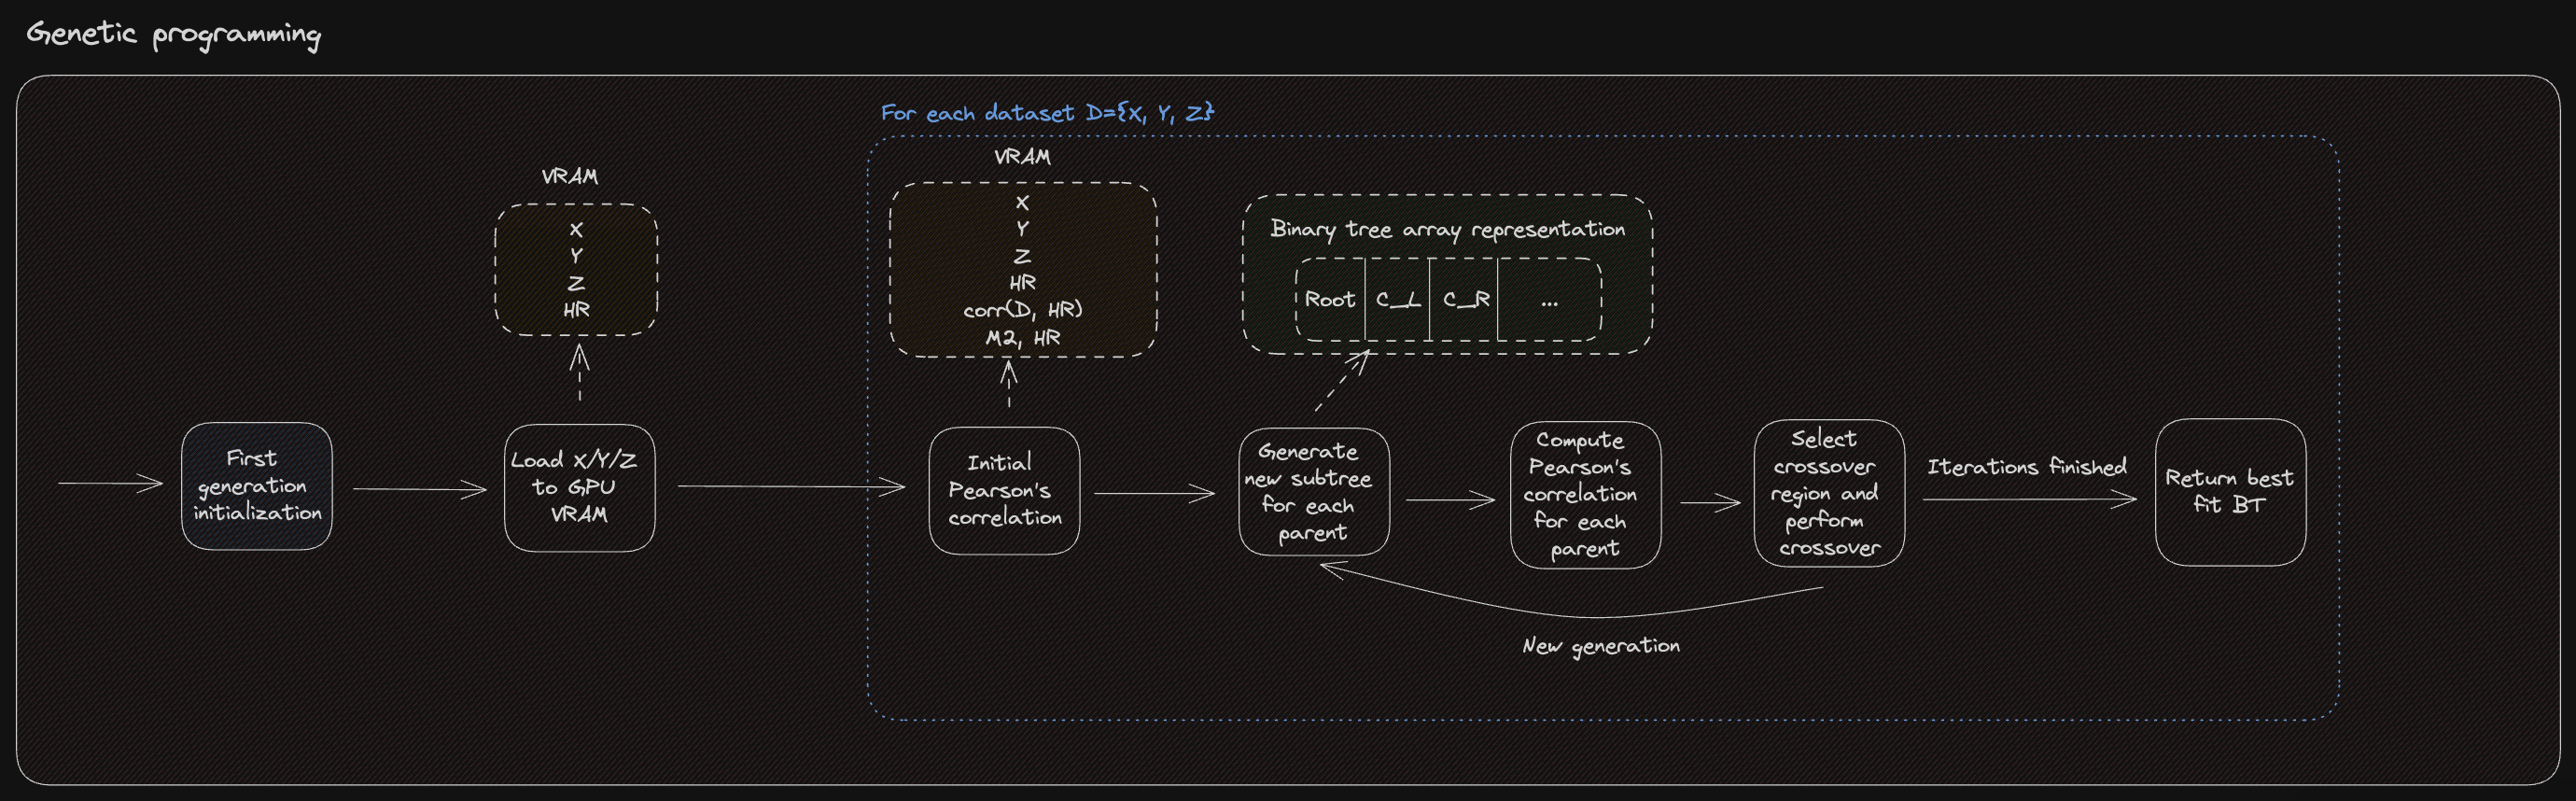
\includegraphics[width=\linewidth]{assets/ppr_diagram_p3.png}
  \caption{Znázornění postupu při výpočtu vzorce korelace}
\end{figure}

\paragraph{} Vypočtenou prvotní korelaci budeme považovat za tzv. \textbf{fitness funkci}. 
Jak bylo řečeno dříve, budeme se snažit o \textbf{minimalizaci rozdílu} nově vypočtené korelace oproti původní.

Výpočet vzorce korelace probíhá celý na vybraném \textbf{OpenCL zařízení}, kromě generace náhodných čísel, které jsou generovány na CPU.
Veškerý výpočet se odehrává v metodě \textit{gpu::GPU::compute\_correlation\_formula}.
Pro připomenutí - algoritmus generuje množinu, kde každý prvek reprezentuje \textbf{úplný binární strom s jedním kořenem a dvěma potomky}. \textbf{Kořen} vždy reprezentuje \textbf{matematickou operaci}, \textbf{listy} vždy reprezentují \textbf{operandy}.
Tyto množiny jsou pak reprezentovány jakožto matice, kde každý řádek reprezentuje právě jednu množinu. 
Množiny jsou vždy stejně velké, jejich velikost je nastavena standardně na \textbf{30}, to znamená, že každá množina obsahuje 10 těchto matematických výrazů.

Prvním krokem je tedy inicializace první generace, která proběhne na CPU.
Velikost generace je nastavena na \textbf{100} jedinců, kdy každá dvojice je inicializována dle popisu na obrázku \ref{fig-starting-generation}.
Poté proběhne inicializace všech potřebných \textbf{OpenCL bufferů}:

\begin{itemize}
  \item Generation buffer - buffer obsahující matici reprezentující celou generaci
  \item ACC buffer - buffer pro naměřené hodnoty v dané ose 
  \item HR values diffs buffer - buffer pro diference rozdílu naměřených hodnot srdečního tepu a jejich průměrné hodnoty (potřebné pro výpočet korelace)
  \item Best fit buffer - buffer pro jedince s nejbližší hodnotou korelace
  \item Best fit values buffer - buffer pro vygenerované hodnoty ,,nejlepším'' jedincem
\end{itemize}

\paragraph{} Po inicializaci bufferů dochází v každé iteraci k následujícím krokům 
\begin{enumerate}
  \item Pro každého jedince vygeneruj nový vektor náhodných čísel respektující jeho reprezentaci (CPU)
  \item Zkopíruj tyto hodnoty do jedince od pozice ,,crossoveru'' do konce pole reprezentující daného jedince (prakticky se přímo modifikuje matice generace)
  \item Proveď ,,crossover'' mezi každou dvojicí jedinců
  \item Vygeneruj nové hodnoty dle vzorce, který jedinec reprezentuje
  \item Vypočti korelaci mezi vygenerovanými a původními hodnotami srdečního tepu
  \item Pokud je korelace bližší té původní, než doposud nejbližší nalezená, považuj tohoto jedince za ,,nejlepšího''
  \item Pokud se v rámci iterace nepodařilo najít lepšího jedince, posuň ,,crossover-point'' blíže konci pole reprezentující jedince
   \begin{itemize}
      \item Operace ,,posun crossover-pointu'' je přidaná implementace pro zlepšení konvergence algoritmu
      \item Uvažuje, že pokud v rámci iteraci nenajdeme lepšího jedince, zkusíme zachovat menší část předka a zakomponovat větší množství mutace do další iterace
      \item V opačném případě uvažujeme, že se blížíme ideálnímu řešení a snažíme se, abychom minimalizovali vliv náhody v další iteraci
   \end{itemize}
 \item Pokračuj krokem 1 po zvolený počet iterací
\end{enumerate}

Veškerý využitý kód pro OpenCL se nachází v souboru \textbf{kernel.cl}.
V tomto zdrojovém souboru se nachází tři využívané funkce. 
První dostupnou funkcí je \textit{generate\_hr\_values}, která jak název napovídá, obsahuje implementaci generování nových hodnot po mutaci a křížení jedinců.
Předchozí kroky, tj. kopírování a ,,crossover'' probíhají za pomocí modifikace a kopírování dat mezi ,,buffery'', pro což OpenCL nabízí metody \textit{enqueueCopyBuffer} a \textit{enqueueWriteBuffer}.
Ve zmíněné metodě pro generování je obsah vektoru reprezentujícího jedince interpretován do příslušného matematického výraz a rovnou vyhodnocen.
Těchto zpracování je nutné provést tolik, kolik je potřeba vygenerovat nových hodnot.
To tedy znamená, že je pro OpenCL tzv. ,,\textbf{NDRange}'' nastaven právě na počet generovaných hodnot a každé výpočetní jádro vygeneruje právě jedno.
Nutno říct, že implementace není optimální, jelikož každé výpočetní jádro musí zpracovat obsah celého jedince.
Zde tedy vnímám prostor pro možnou optimalizaci, když by zpracování jedince bylo delegováno na další výpočetní jádra, tudíž by bylo možné vyhodnocovat veškeré výrazy paralelně, místo sekvenčního zpracování v rámci jedince.
Samozřejmě by bylo nutné zajistit správnou synchronizaci, což by ve výsledku teoreticky mohlo vést jak k lepším, tak horším výsledkům.

Po vygenerování nových hodnot tedy nastává fáze výpočtu korelace mezi těmito a původními hodnotami. 
Výpočet, narozdíl u původní korelace, už taktéž probíhá na OpenCL zařízení pro zajištění minimalizace nutnosti přesouvání dat mezi CPU a OpenCL zařízením (doporučení zadavatele práce).
Jelikož máme veškeré potřebné statistiky původních hodnot srdečního tepu, je potřeba je pouze spočítat pro nově vygenerované hodnoty.
K tomu nám poslouží metoda \textit{calculate\_correlation\_acc\_values}.
Opět platí, že jedno výpočetní jádro zpracovává právě jednu hodnotu pro zajištění maximálního využití poskytnutého OpenCL zařízení.
Nicméně zde narážíme na problém, že je potřeba umět vektor sečíst. 
Na CPU je tato situace v podstatě triviální, nicméně OpenCL standardně nenabízí možnost standardní implementace.
Avšak zde využijeme znalostí z přednášek z předmětu KIV/PPR, kde byla probírána implementace této funkce nazývaná \textbf{parallel prefix sum}.

\begin{figure}
 \centering
  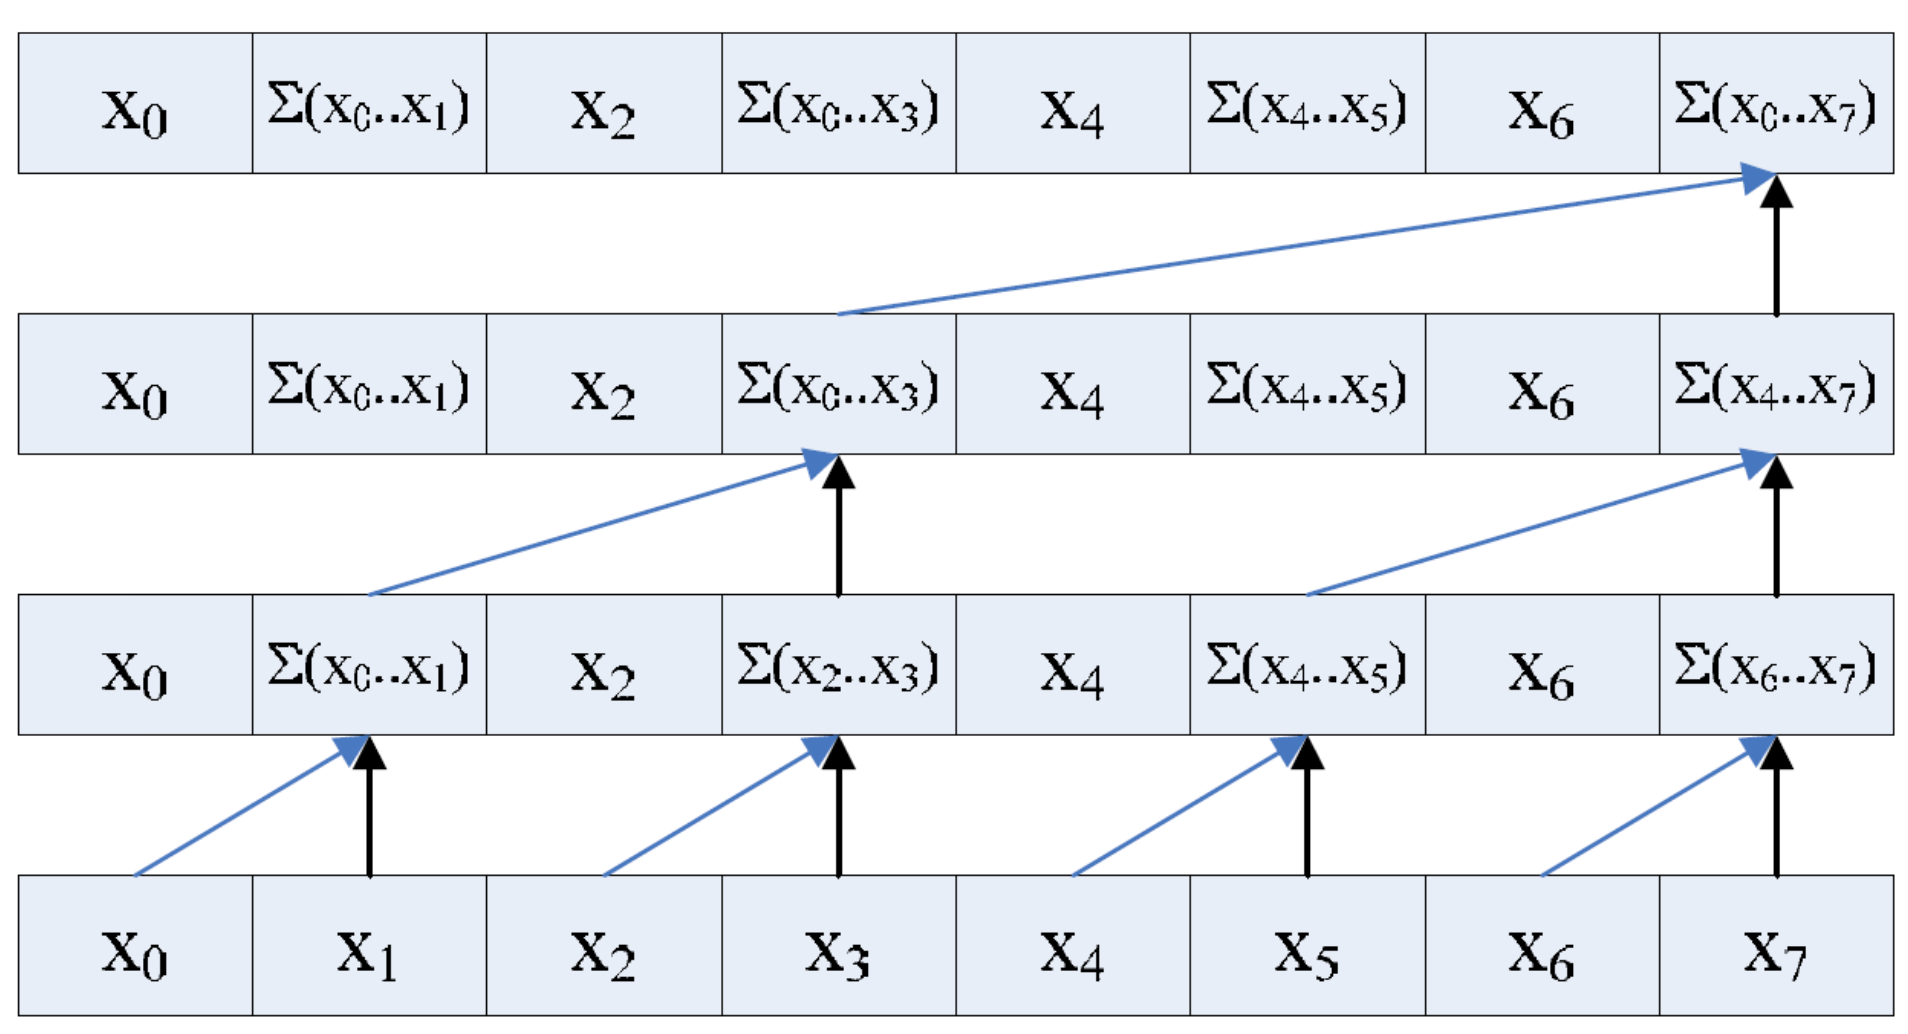
\includegraphics[width=\linewidth]{assets/parallel-prefix-sum.png}
  \caption{Vyobrazení algoritmu ,,parallel prefix sum''. Vyňato z přednášek z předmětu KIV/PPR, zdroj: \href{http://beowulf.lcs.mit.edu/18.337/lectslides/scan.pdf}{odkaz}}
\end{figure}

Nyní tedy máme veškeré prostředky pro úspěšný výpočet ,,nové'' korelace. 
Poté již proběhne několik jednoduchých porovnání a algoritmus končí ve chvíli, kdy se provede zadaný počet iterací (standardně zvoleno \textbf{100}).

\newpage
\section{Výsledky a jejich zhodnocení}
\label{chapter-results}
\paragraph{} Testovací hardware:
\begin{itemize}
  \item PC 1: Desktop, Intel i5 13500 (big.LITTLE, 6P + 8E cores \textrightarrow 20 threads), Intel UHD 770 iGPU, NVIDIA RTX 3060 12GB VRAM, Arch Linux kernel ver. 6.2.8, OpenCL ver. 2.0, GCC 13.2.1
  \item PC 2: MacBook Pro 16 - SoC M1 Pro (10 CPU cores, 16 GPU cores), 16 GB of unified memory, OpenCL ver. 1.2, GCC-13 ver. 13.2.0 (nikoliv Apple Clang wrapper)
\end{itemize}

\paragraph{} Poznámka: Jelikož Apple Clang ve nejnovější verzi k datu tvorby semestrální práce nemá implementované std::execution\_policy pro std::for\_each konstrukt, byla kompilace prováděna za pomocí GNU GCC 13.
Při sestavování pro Apple s Xcode Command Line Tools verze 15.0 je taktéž nutné v rámci parametrů pro linker nutné specifikovat flags \textbf{-Wl,-ld\_classic} (viz \href{https://github.com/Homebrew/homebrew-core/issues/145991}{odkaz}).

\paragraph{} V poskytnutém archivu se výsledky nacházejí ve složce \textbf{results}, spolu s logem z průběhu aplikace pro doložení autentičnosti.
Pro každý subjekt jsou v této složce dostupné 3 grafy ve formátu SVG separátně pro osu X, Y a Z. 
Nad každým grafem se taktéž nachází nalezený vzorec korelace.
Výsledky byly vygenerovány během aplikace na zmíněném Macbook Pro 16.
Kvůli velkému počtu hodnot je v grafu zobrazena každá 10. hodnota.
Nyní se tedy přesuneme ke konkrétním výsledkům:

\begin{itemize}
  \item Subjekt 001 
      \begin{itemize}
        \item X - nalezená korelace 0.229364, v několika úsecích jsou vygenerovaná data velmi blízko původním, avšak zbytek dat se pohybuje spíše pod původními hodnotami
        \item Y - nalezená korelace -0.299763, vygenerovaná data jsou více rozprostřena, menší shoda s původními než pro osu X.
        \item Z - nalezená korelace -0.089666, vygenerovaná data obsahují největší počet téměř shodných úseků s naměřenými daty subjektu 001 
      \end{itemize}
  \item Subjekt 002 
      \begin{itemize}
        \item X - nalezená korelace -0.010386, vygenerovaná data se shodují pouze v jednotkách bodů, zřejmě kvůli nízké korelaci 
        \item Y - nalezená korelace 0.010521, i přes nízkou hodnotu korelace jsou data velmi blízko naměřeným hned v několika úsecích
        \item Z - nalezená korelace -0.211545, data silně mimo trend a rozsah naměřených dat
      \end{itemize}
  \item Subjekt 003 
      \begin{itemize}
        \item X - nalezená korelace -0.194728, vygenerovaná data jeví malou shodu s naměřenými daty
        \item Y - nalezená korelace 0.058434, vygenerovaná data se shodují pouze v jednotkách bodů 
        \item Z - nalezená korelace -0.135090, vygenerovaná data obsahují malý počet úseků částečné shody
      \end{itemize}
  \item Subjekt 004 
      \begin{itemize}
        \item X - nalezená korelace -0.223287, vygenerovaná data obsahují pár úseků částečné shody
        \item Y - nalezená korelace -0.236168, vygenerovaná data obsahují větší počet úseků (než pro osu X) částečné shody s naměřenými daty 
        \item Z - nalezená korelace 0.059885, vygenerovaná data silně mimo trend a rozsah naměřených dat 
      \end{itemize}
  \item Subjekt 005 
      \begin{itemize}
        \item X - nalezená korelace 0.366550, vygenerovaná data mimo spíše trend a rozsah naměřených dat 
        \item Y - nalezená korelace -0.233115, vygenerovaná data obsahují relativně četný počet úseků, ve kterých lze pozorovat částečnou shodu s naměřenými daty  
        \item Z - nalezená korelace -0.191525, vygenerovaná data obsahují relativně četný počet úseků, ve kterých lze pozorovat částečnou shodu s naměřenými daty  
      \end{itemize}
  \item Subjekt 006 
      \begin{itemize}
        \item X - nalezená korelace 0.175462, vygenerovaná data obsahují relativně četný počet úseků, ve kterých lze pozorovat částečnou shodu s naměřenými daty  
        \item Y - nalezená korelace 0.049204, vygenerovaná data obsahují relativně četný počet úseků, ve kterých lze pozorovat částečnou shodu s naměřenými daty  
        \item Z - nalezená korelace -0.204091, vygenerovaná data silně mimo rozsah a trend vůči naměřeným datům
      \end{itemize}
  \item Subjekt 007 
      \begin{itemize}
        \item X - nalezená korelace 0.227925, vygenerovaná data silně mimo rozsah a trend vůči naměřeným datům
        \item Y - nalezená korelace -0.114912, vygenerovaná data obsahují malý počet úseků, ve kterých lze pozorovat částečnou shodu s naměřenými daty 
        \item Z - nalezená korelace -0.198356,  vygenerovaná data obsahují malý počet úseků, ve kterých lze pozorovat částečnou shodu s naměřenými daty 
      \end{itemize}
  \item Subjekt 008 
      \begin{itemize}
        \item X - nalezená korelace 0.358873, vygenerovaná data silně mimo rozsah a trend vůči naměřeným datům 
        \item Y - nalezená korelace -0.226478, vygenerovaná data silně mimo rozsah a trend vůči naměřeným datům 
        \item Z - nalezená korelace 0.101761, vygenerovaná data obsahuji relativně četný počet úseků, ve kterých lze pozorovat částečnou shodu s naměřenými daty 
      \end{itemize}
  \item Subjekt 009 
      \begin{itemize}
        \item X - nalezená korelace -0.165368, vygenerovaná data spíše mimo rozsah a trend vůči naměřeným datům 
        \item Y - nalezená korelace 0.153131, vygenerovaná data obsahují menší počet úseků, ve kterých lze pozorovat částečnou shodu s naměřenými daty 
        \item Z - nalezená korelace 0.083910, vygenerovaná data obsahují relativně četný počet úseků, ve kterých lze pozorovat částečnou shodu s naměřenými daty   
      \end{itemize}
  \item Subjekt 010
      \begin{itemize}
        \item X - nalezená korelace -0.260247, vygenerovaná data obsahují relativně četný počet úseků, ve kterých lze pozorovat částečnou shodu s naměřenými daty 
        \item Y - nalezená korelace 0.055159, vygenerovaná data silně mimo trend a rozsah vůči naměřeným datům  
        \item Z - nalezená korelace -0.060508, vygenerovaná data obsahují relativně četný počet úseků, ve kterých lze pozorovat částečnou shodu s naměřenými daty 
      \end{itemize}
  \item Subjekt 011
      \begin{itemize}
        \item X - nalezená korelace -0.063953, vygenerovaná data obsahují relativně četný počet úseků, ve kterých lze pozorovat částečnou shodu s naměřenými daty 
        \item Y - nalezená korelace -0.269928, vygenerovaná data obsahují menší počet úseků, ve kterých lze pozorovat částečnou shodu s naměřenými daty 
        \item Z - nalezená korelace -0.259825, vygenerovaná data silně mimo trend a rozsah vůči naměřeným datům  
      \end{itemize}
  \item Subjekt 012
      \begin{itemize}
        \item X - nalezená korelace -0.077606, vygenerovaná data silně mimo trend a rozsah vůči naměřeným datům, neobvykle nízký počet vygenerovaných vzorků
        \item Y - nalezená korelace -0.183245, vygenerovaná data silně mimo trend a rozsah vůči naměřeným datům 
        \item Z - nalezená korelace -0.238987, vygenerovaná data obsahují menší počet úseků, ve kterých lze pozorovat částečnou shodu s naměřenými daty 
      \end{itemize}
  \item Subjekt 013
      \begin{itemize}
        \item X - nalezená korelace -0.455067, vygenerovaná data obsahují menší počet úseků, ve kterých lze pozorovat částečnou shodu s naměřenými daty 
        \item Y - nalezená korelace 0.085192, vygenerovaná data obsahují relativně četný počet úseků, ve kterých lze pozorovat částečnou shodu s naměřenými daty 
        \item Z - nalezená korelace -0.417171, vygenerovaná data silně mimo trend a rozsah vůči naměřeným datům  
      \end{itemize}
  \item Subjekt 014
      \begin{itemize}
        \item X - nalezená korelace -0.172943, vygenerovaná data silně mimo trend a rozsah vůči naměřeným datům  
        \item Y - nalezená korelace 0.243723, vygenerovaná data obsahují relativně četný počet úseků, ve kterých lze pozorovat částečnou shodu s naměřenými daty 
        \item Z - nalezená korelace -0.174381, vygenerovaná data obsahují menší počet úseků, ve kterých lze pozorovat částečnou shodu s naměřenými daty 
      \end{itemize}
  \item Subjekt 015
      \begin{itemize}
        \item X - nalezená korelace 0.084257, vygenerovaná data spíše mimo rozsah a trend vůči naměřeným datům, možná degradace genetického algoritmu
        \item Y - nalezená korelace -0.054542, vygenerovaná data spíše mimo rozsah a trend vůči naměřeným datům, možná degradace genetického algoritmu
        \item Z - nalezená korelace -0.399695, vygenerovaná data spíše mimo rozsah a trend vůči naměřeným datům, možná degradace genetického algoritmu
      \end{itemize}
  \item Subjekt 016
      \begin{itemize}
        \item X - nalezená korelace 0.187688, vygenerovaná data silně mimo trend a rozsah vůči naměřeným datům  
        \item Y - nalezená korelace -0.262219, vygenerovaná data obsahují menší počet úseků, ve kterých lze pozorovat částečnou shodu s naměřenými daty 
        \item Z - nalezená korelace -0.118415, vygenerovaná data spíše mimo rozsah a trend vůči naměřeným datům
      \end{itemize}
\end{itemize}

\paragraph{} Na základě výše uvedených závěrů lze pozorovat, že ve většině případů byly naměřený dvě záporné a jedna kladná korelace, což se dá považovat za očekávané.
U subjektu 15 se zdá, že došlo k degradaci genetického algoritmu na základě příslušných grafů. 
Celkově se tedy bohužel nepovedlo nalézt jednoznačnou shodu mezi naměřenými daty a nalezeným vzorcem pro korelaci, nicméně se z hodnot zdá, že zde malá závislost existuje.

\newpage
\section{Závěr}
\paragraph{} Podařilo se mi tedy vytvořit aplikaci dle požadavků zadání, která pomocí genetického algoritmu a využití technik paralelního programování hledá vzorec pro nalezení korelace mezi naměřenými daty.
I přes časově náročnou analýzu problému a implementace se stále jedná o relativně pomalý běh (celkově zhruba 20 minut), nicméně byly identifikovány tzv. ,,bottlenecky'' a návrh jejich zlepšení, tudíž stále existuje prostor pro zlepšení.
Bohužel, z časových důvodů již nebylo možné tyto návrhy zapracovat do finálního řešení. 
Samotná tvorba semestrální práce (včetně analýzy) započala 25.9.2023 a finální verze byla dokončena dne 31.12.2023.
Celkově bylo na semestrální práce stráveno zhruba 296 hodin čistého času, včetně veškerých potřebných souvisejících úkonů (jako například studování podkladů, analýza, programování, dokumentace, \dots).

Na úplný závěr bych rád sdělil pár slov z hlediska osobních pocitů ohledně předmětu KIV/PPR. 
Díky této práci jsem nabyl nových nedocenitelných zkušeností ohledně faktu, že kvalitní analýza je \textbf{VŽDY} důležitá a ve výsledku může značně usnadnit práci při samotném vývoji.
Dále jsem velmi potěšen přístupem pana doc. Ing. Tomáše Koutného, Ph.D. se zábavnými, a zároveň velmi naučnými přednáškami.
Předmět mi nadále poskytl absolutně zásadní zajímavosti a znalosti ohledně obecného, efektivního a výkonově závislého programování, v čemž osobně díky tomuto předmětu nalézám zálibu. 
Osobně jsem tedy velmi rád, že jsem si předmět zapsal i přes to, že je jeho látka koncepčně velmi náročná.  


\newpage
\bibliographystyle{unsrt}
{\raggedright\small
\bibliography{literatura}
}

\end{document}

